\documentclass[a4paper]{article}
\usepackage[T1]{fontenc}
\usepackage[utf8]{inputenc}
\usepackage[siunitx]{circuitikz}
\usepackage{siunitx}
\usepackage[margin=2cm]{geometry}
\usepackage{systeme}
\usepackage{mathtools}
\usepackage{wrapfig}
\usepackage[export]{adjustbox}
\usepackage{subcaption}
\usepackage{pdfpages}
\usetikzlibrary{calc}

\usepackage[swedish]{babel}
 % Needed for the Swedish characters



%TODO fix voltage over L_1!!!

\title{Inlämningsuppgift 2-1045}
\author{Oskar Philipsson}
\index{}
\begin{document}

\begin{titlepage}
\maketitle

\end{titlepage}
\tableofcontents
\section{Intro}
\subsection{Uppgift}

\includepdf[pages={2}]{elektronikuppgifter.pdf}

\subsection{Avritat kretsschema}

\begin{figure}[h]
\begin{circuitikz}[american, scale=0.8, /tikz/circuitikz/bipoles/length=1cm] \draw
(0,0) to[sI=$i_0(t)$ ]++(0,4)
to[short,-*]node[label = A](A){}++(3,0)
--++(8,0) --++(0,-1)
node[transformer,anchor=A1](T){}
(T.A2) |- (3,0)node[label = B](B){}
to[short,*-]++(-3,0)
%(T.inner dot A1) node[circ]{}
%(T.inner dot B1) node[circ]{}

++(2,4) to[generic,l_=$Z_i$]++(0,-4)
++(2,4) to[R,l_=$R_1$,a^=1<\kilo\ohm>]++(0,-4)
++(3,4) to[R,l_=$R_2$,a^=1<\kilo\ohm>]++(0,-2)
to[C,l_=$C_1$,a^=2<\micro\farad>]++(0,-2)
++(3,4) to[C,l_=$C_2$,a^=1<\micro\farad>]++(0,-4)
;
\draw(T.B1)-- ++(0,1)--++(6,0)
to[L,l_=$L_1$,a^=10<\milli\henry>]++(0,-4)--++(-3,0)
++(4.5,4)to[open,v^=$u(t)$]++(0,-4)to[open]++(-4.5,0)
to[R,l=$R_3$,a=10<\ohm>]++(0,4)
++(0,-4)--++(-3,0)--(T.B2)
(A) to[open] (B)
;
\end{circuitikz}
\caption{Avritat kretsschema}
\label{fig:orginal}
\end{figure}


\subsection{Symbolförklaringar}

\begin{figure}[h]
 
\begin{subfigure}{0.333\textwidth}
\begin{circuitikz} [american]\draw
(0,0) to[V,l^=$E_1$, a_=3<\volt>](4,0)
;
\end{circuitikz}
\caption{Spänningskälla}
\end{subfigure}
%
\begin{subfigure}{0.333\textwidth}
\begin{circuitikz} [american]\draw
(0,0) to[current source, l^=$I_{01}$,a_=1<\milli\ampere>](4,0)
;
\end{circuitikz}
\caption{Strömkälla}
\end{subfigure}
%
\begin{subfigure}{0.333\textwidth}
\begin{circuitikz} \draw
(0,0) to[R,l^=$R_2$,a_=2k](4,0)
;
\end{circuitikz}
\caption{Resistans}
\end{subfigure}
 
\end{figure}

Alla komponenter antas vara ideala. Spänningskällan har högre potential på sidan med plustecknet. Strömkällan driver en ström i pilens riktning. Komponenters värden betecknas med $E_n, I_{0n}, R_n$ för spänning, ström respektive resistans. Komponenternas värden står tydligt utmarkerade vid respektive komponent med dess värde på andra sidan komponenten.
Strömmen $I_n$ betecknar strömmen som går mellan två noder, förutom de som kommer direkt från en strömkälla vilka betecknas $I_{0m}$. Vardera strömm betecknas enbart en gång. 
Beteckningen $V_k$ används för potentialen i noden som beteckningen står vid.

\section{Förenkling av kretsschema}

Jag börjar med att ersätta strömkällan och dess inre resistans med en spänningskälla och den inre resistansen i serie. Detta får jag göra då de båda delkretsarna är antigen en Nortonekvivalent eller en Theveninekvivalent, vilket gör att kretsarna blir ekvivalenta. Sedan skriver jag om allt till komplex form och använder $j\omega$-metoden. Den omtalade spänningskällan får då värdet $E = Z_iI = 100e^{j\frac{\pi}{4}} \cdot 0.01 = e^{j\frac{\pi}{4}} V$ Detta illustreras i följande schema.

% Komplext schema------------------------------------------------
\begin{circuitikz}[american, scale=0.8, /tikz/circuitikz/bipoles/length=1cm] \draw
(0,0) to[esource ,v<=$E$]++(0,4)
to[generic,l_=$Z_i$,-*]++(3,0)node[label=A](A){}
--++(8,0) --++(0,-1)node(test){} 
node[transformer,anchor=A1](T){}
(T.A2) |- (3,0)node[label = B](B){}
to[short,*-]++(-3,0)
%(T.inner dot A1) node[circ]{}
%(T.inner dot B1) node[circ]{}
++(5,4) to[generic,l_=$R_1$]++(0,-4)
++(2,4) to[generic,l_=$R_2$]++(0,-2)
to[generic,l_=$\frac{1}{j \omega C_1}$,a^=]++(0,-2)
++(3,4) to[generic,l_=$\frac{1}{j \omega C_2}$]++(0,-4)
;
\draw(T.B1)-- ++(0,1)--++(6,0)
to[generic,l_=$j \omega L_1$]++(0,-4)--++(-3,0)
++(4,4)to[open,v^=$U$]++(0,-4)to[open]++(-4,0)
to[generic,l=$R_3$]++(0,4)
++(0,-4)--++(-3,0)--(T.B2)

;
\end{circuitikz}

Sedan föreklar kretsen till följande.

% Förenklat med transformator------------------------------------------------
\begin{circuitikz}[american, scale=0.8, /tikz/circuitikz/bipoles/length=1cm] \draw
(0,0) to[esource ,v<=$E$]++(0,4)
to[generic,l_=$Z_i$,-*]++(3,0)node[label=A](A){}
--++(4,0) --++(0,-1)node(test){} 
node[transformer,anchor=A1](T){}
(T.A2) |- (3,0)node[label=B](B){}
to[short, *-](0,0)
%(T.inner dot A1) node[circ]{}
%(T.inner dot B1) node[circ]{}

++(5,4) to[generic,l_=$Z_{e1}$]++(0,-4)
;
\draw(T.B1)-- ++(0,1)--++(3,0)
to[generic,l_=$Z_t$]++(0,-4)
++(4,4)to[open,v^=$U$]++(0,-4)to[open]++(-4,0)
-|(T.B2)

;
\end{circuitikz}

Detta ger 
\begin{equation}
    Z_{e1} = R_1 // (R_2 + \frac{1}{j \omega C_1})//\frac{1}{j \omega C_2} \quad \Rightarrow \quad \\
    \frac{1}{Z_{e1}} = \frac{1}{R_1} + \frac{1}{(R_2 + \frac{1}{j \omega C_1}})+ j \omega C_2 \quad \Rightarrow \quad \\
    Z_{e1} = hitta i matlab
\end{equation}

och 

\begin{equation}
    \frac{1}{Z_t} = \frac{1}{R_3} + \frac{1}{j \omega L_1} \quad \Rightarrow \quad \\
    Z_t = hitta i matlab
\end{equation}

Transformatorn och $Z_t$ kan ersättas enligt följande. $Z'_t = \left(\frac{N_1}{N_2}\right)^2 Z_t = hitta i matlab$. Se REF TEST.
% Förenklat utan transformator------------------------------------------------
\begin{circuitikz}[american, scale=0.8, /tikz/circuitikz/bipoles/length=1cm] \draw
(0,0) to[esource ,v<=$E$]++(0,4)
to[generic,l_=$Z_i$,-*]++(3,0)node[label=A](A){}
--++(4,0)
to[generic,l=$Z'_t$]++(0,-4) 
--(3,0)node[label=B](B){}
to[short, *-](0,0)

++(5,4) to[generic,l_=$Z_{e1}$]++(0,-4)
(A)to[open]++(0,-0.5)to[open, v=$U_{ab}$] ++(0,-3)
;

\end{circuitikz}

Nu ersätts $Z_{e1} // Z'_t med Z_{e2} = \frac{Z_{e1} Z'_t}{Z_{e1} + Z'_t} = HITTA I MATLAB$

Spänningen $U_{ab}$ får genom spänningsdelning. $U_{ab} = \frac{Z_{e2} U_0}{Z_{e2} + Z_i} = HITTA I MATLAB$ Spänningen $U$ fås genom spänningsformel för ideal transformator som i detta fallet är $\frac{u_1}{u_2} = \frac{N_1}{N_2} \quad \Rightarrow \quad U = \frac{U_{ab}}{\frac{N_1}{N_2}} = HITTA I MATLAB$

\section{B}

Reaktiv effekt fås enligt $Q = X I_e^2$ och aktiv effekt enligt $P = R I_e^2$. $I_e = \frac{1}{\sqrt{2}}\left|\frac{U}{Z_t}\right| = HITTA I MATLAB$. Detta ger $Q = HITTA I MATLAB$ och $P = HiTTA I MATLAB$.

\section{C}
Maximal effektutveckling erhålls då $z_e2 = Z_i^*$


\end{document}